\documentclass[conference]{IEEEtran}
\IEEEoverridecommandlockouts
% The preceding line is only needed to identify funding in the first footnote. If that is unneeded, please comment it out.
\usepackage{cite}
\usepackage{amsmath,amssymb,amsfonts}
\usepackage{algorithmic}
\usepackage{graphicx}
\usepackage{textcomp}
\usepackage[table]{xcolor}
\usepackage{xurl}
\usepackage{hyperref}
\usepackage{ragged2e}
\usepackage{caption}
\usepackage[utf8]{inputenc}
\usepackage[english]{babel}


\usepackage{listings}
\lstset{language=[LaTeX]TeX,breaklines=true} % Word wrap within listings environment
\definecolor{codegreen}{rgb}{0,0.6,0}
\definecolor{codegray}{rgb}{0.5,0.5,0.5}
\definecolor{codepurple}{rgb}{0.58,0,0.82}
\definecolor{backcolour}{rgb}{0.95,0.95,0.92}

% defines code block style 
\lstdefinestyle{mystyle}{
    backgroundcolor=\color{backcolour},   
    commentstyle=\color{codegreen},
    keywordstyle=\color{magenta},
    numberstyle=\tiny\color{codegray},
    stringstyle=\color{codepurple},
    basicstyle=\ttfamily\footnotesize,
    breakatwhitespace=false,         
    breaklines=true,                 
    captionpos=b,                    
    keepspaces=true,                 
    numbers=left,                    
    numbersep=5pt,                  
    showspaces=false,                
    showstringspaces=false,
    showtabs=false,                  
    tabsize=2
}
\lstset{style=mystyle,columns=fullflexible}




\usepackage[
backend=biber,
style=numeric,
sorting=ynt
]{biblatex}
\addbibresource{research.bib}

\def\BibTeX{{\rm B\kern-.05em{\sc i\kern-.025em b}\kern-.08em
    T\kern-.1667em\lower.7ex\hbox{E}\kern-.125emX}}
\begin{document}


\title{Hardware Accelerated QC-MDPC McEliece Cryptosystem\\
}

\author{\IEEEauthorblockN{Dzurick, Mitchell}
\IEEEauthorblockA{\textit{Eletrical and Computer Engineering} \\
\textit{University of Arizona}\\
Tucson, Arizona \\
mitchdz@email.arizona.edu}
\and
\IEEEauthorblockN{Russell, Mitchell}
\IEEEauthorblockA{\textit{Electrical and Computer Engineering} \\
\textit{University of Arizona}\\
Tucson, Arizona \\
mcrussell@email.arizona.edu}
\and
\IEEEauthorblockN{Kuban, James}
\IEEEauthorblockA{\textit{Electrical and Computer Engineering} \\
\textit{University of Arizona}\\
Tucson, Arizona \\
kubandj@email.arizona.edu}
}

\maketitle

\begin{abstract}
    \colorbox{yellow}{NOTE: 100-150 characters}
    Due to the advent of quantum computers, a need for new cryptographic algorithms that can resist this new computing type emerged. Classic logarithmic based algorithms such as AES and RSA are hard for classical computers to crack, but not as challenging for quantum computers, the McEliece cryptosystem is one of them. The McEliece cryptosystem linearly expands the message and intentionally adds errors to be recovered later. To achieve this, many matrix operations are performed on large matrices which is very demanding for a CPU. This paper focuses on using CUDA with a dedicated graphics card to accelerate the time to perform encryption and decryption with the McEliece cryptosystem. The resulting cryptosystem has an overall end-to-end speedup of 8.89X. This speedup renders the McEliece cryptosystem more realistic for actual use.
\end{abstract}

\begin{IEEEkeywords}
    CUDA, McEliece, cryptography
\end{IEEEkeywords}

\section{Introduction}\label{Introduction}
    \colorbox{yellow}{TODO: Introduction}
    % why should I read this paper?
    
    % motivation
    The McEliece cryptosystem is one of the many proposed post-quantum asymmetric encryption algorithms. The McEliece cryptosysem is resistant to Shor's algorithm which means that quantum computers can not brute-force the decryption keys in polynomial time. 
    % problem statement
    The McEliece algorithm specifies a small list of steps in order to generate cipher text that can be recovered. This paper aims to improve the execution time of a Quasi Cyclic-Moderate Density Parity Check (QC-MDPC) based McEliece cryptosystem in key generation, encryption, and decryption. This implementation of the McEliece cryptosystem involves very large matrix operations in all steps of the program. The paper shows how a speedup of \textbf{9614X} for matrix multiplication, \textbf{9.08X} for matrix addition, and \textbf{3.46X} for matrix inverse was achieved to get an overall speedup of \textbf{13.32X}.
    
    


\section{Related Work}\label{Related Work}
    The C based code that this project is based off is the McEliece cryptosystem created by Varad0612 \cite{varad0612}.
    \colorbox{yellow}{TODO: add more references, especially with OpenMP}


\section{Background}\label{Background}
    The Mceliece cryptosystem is a relatively simple system to understand. Figure~\ref{fig:linear expansion} shows a top level view of the cryptosystem. There are two main steps to the system, linearly expanding the plaintext, and then intentionally adding errors that can be recovered later.

    \subsection{Top Level View}\label{Top Level View}
        \begin{center}
            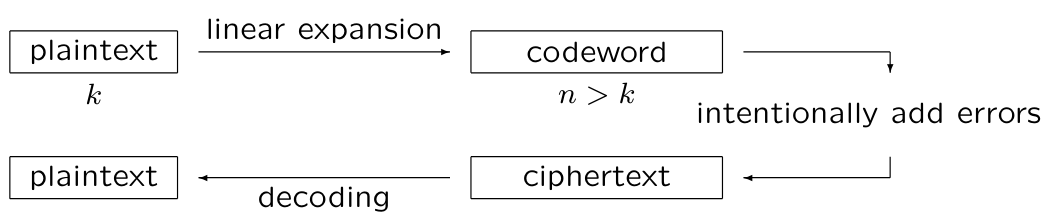
\includegraphics[width=0.45\textwidth]{Linear_Expansion.png}
            \\Source: nist.gov
            \captionof{figure}{McEliece top level view}
            \label{fig:linear expansion}
        \end{center}
        
    
        There are a few versions of the McEliece cryptosystem, and for this paper we are reviewing the QC-MDPC (Quasi Cyclic - Moderate Density Parity Check) variant of the cryptosystem. The QC-MDPC McEleice cryptosystem takes four inputs, $n$, $p$, $t$, and $w$ where
    
        \begin{enumerate}
            \item $n$ is the length of the error vector
            \item $p$ is the dimension of the private/public key
            \item $t$ is the weight of the error matrix
            \item $w$ is the weight of the QC MDPC code
        \end{enumerate}
        
        The effective keyspace, $k$ is $\{0,1\}^{(n-1)*p}$. This keyspace is what determines how much data you can encrypt. If the size of your data is less than $k$ then you will not be able to use this cryptosystem. Therefore, for larger sized files you are required to adjust your input parameters appropriately.
    \subsection{McEliece Operations}\label{McEliece Operations}
        The McEliece cryptosystem offers support to \textbf{generate a pair of asymmetric keys}, \textbf{encrypt}, and \textbf{decrypt} data. This paper does not aim to explain the rational or the math behind each operation, but rather to show the the process involved with each operation.
    
        \textbf{Key Generation:}\label{Key Generation} \\
            Key generation starts with creating the private key, \textbf{H} which is a parity-check matrix. This paper will not go into how \textbf{H} is generated, because the process is very serialized, but does not take that long on a CPU. The key that is worth looking into is the public key \textbf{G}.
            
            \begin{center}
                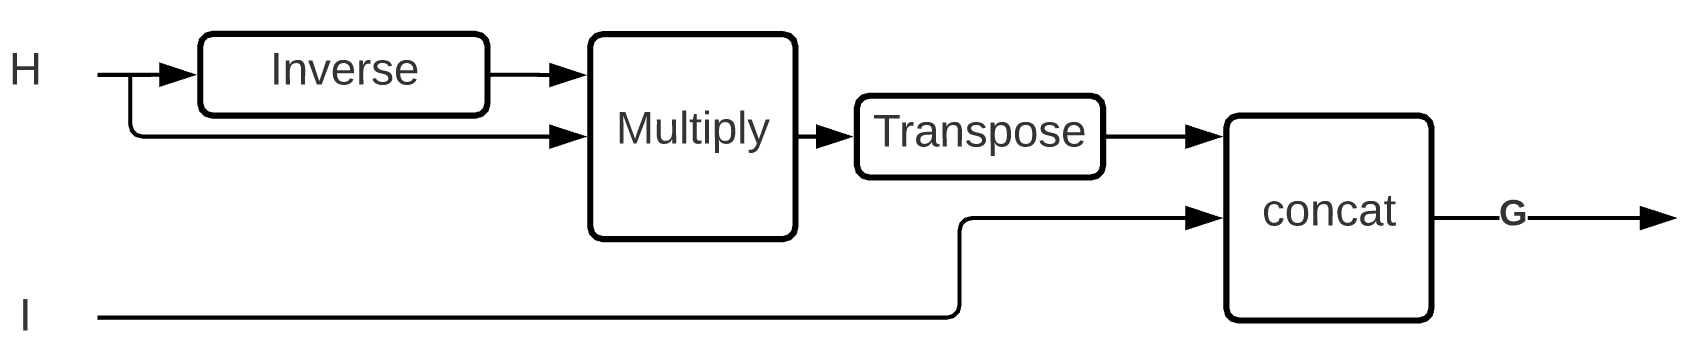
\includegraphics[width=0.45\textwidth]{Keygen.png}
                \captionof{figure}{McEliece Keygen Diagram}
                \label{fig:keygen}
            \end{center}          
            
            Figure~\ref{fig:keygen} shows the resulting operations needed the generate the public key \textbf{G}. It can be seen that 3 expensive matrix operations are needed: inverse, multiply, and transpose. The matrix \textbf{I} is the identity matrix of size H.
            
            
        \textbf{Encryption:}\label{Encryption} \\
            compute the ciphertext c as
            \begin{equation} \label{eq:encryption}
                      c = uG + e
            \end{equation}
    
            where $u$ is the plaintext, $G$ is the generator matrix, and $e$ is an error vector.
        
            \begin{center}
                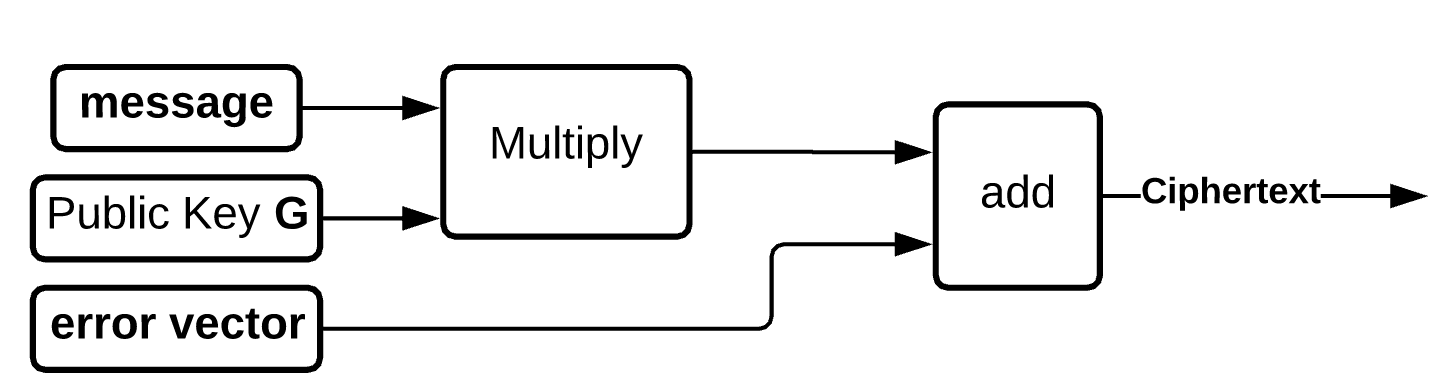
\includegraphics[width=0.45\textwidth]{Encryption.png}
                \captionof{figure}{McEliece Encryption Diagram}
                \label{fig:encryption}
            \end{center}        
        
            figure~\ref{fig:encryption} shows a diagram of the operations needed to encrypt a message. The two multiply and add operations are matrix operations, thus they slow down a lot when the key sizes are very large.
        
        
        \textbf{Decryption:}\label{Decryption} \\
            To decrypt a ciphertext $c$, the user has to obtain the private key \textbf{H}. The decryption function has to be some type of decoding function that can recover the errors intentionally added during the encryption process. This implementation of the McEliece cryptosystem uses \textit{syndrome decoding}. This paper does not aim to explain syndrome decoding, so a function $DEC_{H}(c)$ is defined as the syndrome decoding function, which requires the private key \textbf{H} and the ciphertext $c$

            \begin{equation} \label{eq:decryption}
                      u = DEC_{\textbf{H}}(c)
            \end{equation}
            
            Where u is the plaintext, \textbf{H} is the private key, and c is the ciphertext generated from Equation~\ref{eq:encryption}. This paper will not go into syndrome decoding as that is out-of-scope (for the sake of time), but do know that in the process of setting up syndrome decoding, matrix multiplication and matrix addition are used.

    \subsection{Binary Arithmetic}
        Because McEliece is a binary encoding based cryptosystem, every matrix operation is not floating point arithmetic, but rather binary arithmetic. This causes a few annoyances because most standard libraries do not handle binary arithmetic. For example, CuBLAS only handles floating point arithmetic for matrix inverse operations.

    \subsection{Functional Security}
        It is important to pick the right input parameters to this cryptosystem to try and achieve the desired security. It is often referenced that a certain set of input parameteres offer a level of security in bits\cite{10.1109/ISIT.2013.6620590, 10.1007/978-3-642-29011-4_31}. what this means is that for example if you have a level of security of 80 bits, it will take $2^{80}$ computations to brute-force the secret key. Determining the realistic security of this cryptosystem is more nuanced than simple thinking about the input parameters, but for this paper we aim to find a generalized baseline to hopefully achieve a realistic implementation in a reasonable amount of time. 
        
        To determine the security of the system, we must determine the most effective way of attacking the cryptosystem currently known. At the time of writing this paper, it is believed that Information Set Decoding (ISD) is the most effective attack against this cryptosystem. Anja Becker, et. al. Explain the challenges of ISD and propose an algorithm to attack this cryptosystem in asymptotic computational complexity\cite{10.1007/978-3-642-29011-4_31}. 
        
        This asymptotic computational complexity is what is referenced when a certain set of input parameters is considered. \colorbox{yellow}{TODO: input param to bits of security}





\section{Methodology}\label{Methodology}
    The goal of this project is to convert a CPU-based cryptosystem into one that can leverage hardware acceleration. Therefore, we want the operations of the system to remain very close to the source code. The obvious first choice is to review the source code, and find functions that are optimal for GPU based execution. After doing initial research, the following kernels were determined to be the most time consuming and worth-while to convert to CUDA:
    
    \begin{enumerate}
        \item Matrix Multiplication
        \item Matrix Transpose
        \item Matrix Inverse
        \item Matrix Addition
    \end{enumerate}
    
    The matrix operations mentioned above are the largest bottleneck for CPU execution, as the matrix operations required for this cryptosystem are very large and take an unreasonable amount of time for a CPU based execution.
    
    
    
    \colorbox{yellow}{TODO: expand}

\section{Evaluation and Validation}\label{Evaluation and Validation}
    Evaluation on the created system is directly compared to the C based implementation. The system that all tests were ran on has 16GB of DDR4 RAM, Intel(R) Core(TM) i9-9900KF CPU @ 5.0GHz, and a GTX 980Ti. Evaluation was done on each major matrix operation via timing analysis, comparing directly to the C based implementation. Validation was relatively straight-forward where we created a kernel (or set of kernels) to achieve the same functionality as a function in the baseline code. If the kernel or sets of kernels produced the same output as the baseline C code, it is validated to work properly. Each test-case requires different input parameters, but testing was done with the goal of realistic operations that the cryptosystem would encounter. For example, there would not be any need to test a matrix operation on rectangular test inputs when the code only works on square matrices.
    
    \subsection{Experimental Results and Analysis}\label{Experimental Results and Analysis}
        Experimental results consist of timing analysis for each major matrix operation that was targetted to be sped up, and an overall end-to-end testk that includes generating a pair of keys, encrypting random data, and decrypting random data.
            
            
            
        \paragraph{Matrix Multiplication Kernel}\label{Matrix Multiplication Kernel}\\
        
            \colorbox{yellow}{TODO: add table of timing}
            
            \begin{center}
                {\rowcolors{2}{green!80!yellow!50}{green!70!yellow!40}
                \begin{tabular}{ | c | c | c | c | } \hline
                    \shortstack{matrix\\dimension} & \shortstack{CPU\\(seconds)} & \shortstack{GPU\\(seconds)} & \shortstack{Optimized GPU \\(seconds)}\\ \hline
                    16 & 0 & 0.16 & 0 \\ \hline
                    32 & 0 & 0.12 & 0 \\ \hline
                    64 & 0 & 0.12 & 0 \\ \hline
                    128 & 0.01 & 0.12 & 0 \\ \hline
                    256 & 0.07 & 0.12 & 0 \\ \hline
                    512 & 0.56 & 0.13 & 0 \\ \hline
                    1024 & 4.46 & 0.11 & 0 \\ \hline
                    2048 & 35.55 & 0.14 & 0.01\\ \hline
                    4096 & 283.79 & 0.23 & 0.04 \\ \hline
                    8092 & 2307.38 & 0.9 & 0.24\\ \hline
                    16384 & N/A & 5.99 & 1.71\\ \hline
                    32768 & N/A & 46.08 & 12.53\\ \hline
                \end{tabular}
                }
                \captionof{table}{Timing results for Matrix Multiplication execution}
                \label{fig:E2E_table}
            \end{center}

            
            
            
        \textbf{Matrix Inverse}\label{Matrix Inverse}\\
        \colorbox{yellow}{TODO: add table of timing}
            
        Matrix Inversion is a very serialized task, the common Gaussian elimination requires many operations that depend on previous operations. This is not ideal for a GPU when we want to be able to do all operations in parallel. Therefore, in order to do matrix inversion on a GPU, LU decomposition was created to be used instead of regular Gaussian elimination.
            
        LU Decomspotion is not a single kernel, but rather a string of kernels doing specific tasks. The following kernels were created to allow GPU based LU decomposition:
        \begin{itemize}
            \item GF2\_LU\_decompose\_find\_max\_row
            \item GF2\_LU\_decompose\_update\_trailing\_row 
            \item make\_GF2\_identity\_gpu
            \item GF2\_Forward\_substitute
            \item GF2\_Backward\_substitute
            \item GF2\_swap\_cols
        \end{itemize}

        Each kernel has a specific task, and the order of which they are called is important. To reduce the latency of generating an identity matrix, a single threadblock is dedicated to run in parallel with all of the decomposition steps. This means that once decomposition is done, the program can immediately start performing forward substitution. This is achieved through the use of CUDA streams.
        
        
        \textbf{GF2\_LU\_decompose\_find\_max\_row} kernel is unfortunately single threaded because it just does a linear search and returns as soon as it finds a one in the current row's sub-diagonal. This means that if the parity check matrix is more dense, then this function returns a lot faster. 
        
        
        \textbf{GF2\_LU\_decompose\_update\_trailing\_row } kernel is the longest kernel in the decompose kernels. This kernel has to update the current row and every row below it. What makes this kernel really inefficient is that each row that the program goes down, the program updates less values. That means that more threads are idle on the later rows to be updated. With that said, this kernel is being sped up greatly by having a single thread handle each column element.
        
        
        \textbf{make\_GF2\_identity\_gpu} kernel is a kernel mentioned earlier that is meant to be called with a single threadblock. This kernel is designated to use a different cuda stream than the rest of the decompose kernels, and therefore gets generated slowly while decomposing the matrix. Usually, there is a delay after you are done decomposing to generate the matrix, and this speeds that up. The only downside to this method is that if the decompose steps requires all available threadblocks to operate, then this kernel could slow the program down.
        

        \textbf{GF2\_Forward\_substitute} kernel 


        \textbf{GF2\_Backward\_substitute} Kernel is really similar to the forward substitution kernel. Each thread handles a separate column value.


        Profiling was done on each kernel, but unfortunately no interesting information was gained through the use of profiling. The weak points in each kernel were already known before profiling. In addition to that, profiling the overall inverse function is an extremely timely process as nvprof has the rewind each kernel call. There are 4 + N*3 kernel calls where N is the dimension of the square matrix. Therefore, it could take hours to profile an execution time that only took a few minutes.
        
        
        
        \colorbox{yellow}{TODO: fix table timing}
        \begin{center}
            {\rowcolors{2}{green!80!yellow!50}{green!70!yellow!40}
            \begin{tabular}{ | c | p{1.2cm} | p{1.2cm} | p{1.2cm} | p{1.2cm} | } \hline
                \shortstack{matrix\\dimension} & \shortstack{CPU GJ\\(seconds)} & \shortstack{CPU LU\\(seconds)} & \shortstack{GPU LU\\(seconds)} & speedup\\\hline
                512 & 0.19 & 0.43 & 0.57 & 0.34\\ \hline
                1024 & 1.43 & 4.43 & 3.19 & 0.45\\ \hline
                2000 & 11.43 & 26.29 & 12.38 & 0.90\\ \hline
                3050 & 11.43 & 26.29 & 12.38 & 0.95\\ \hline
                4000 & 37.00 & 269 & 44.96 & 1.19\\ \hline
                4400 & 42.70 & N/A & 39.60 & 1.08\\ \hline
                6000 & 375 & 1010.7 & 132.49 & 2.84\\ \hline
                12000 & 862.2 & 8927.2 & 249.0 & \textbf{3.46}\\ \hline
                24000 & 8638 & N/A & 4172 & 2.07\\ \hline
            \end{tabular}
            }
            \captionof{table}{Timing results for Inverse Matrix execution}
            \label{fig:inverse_table}
        \end{center}

        Table~\ref{fig:inverse_table} shows the timing results, with the execution time of CPU based LU decomposition added in. It can be seen that the CPU based LU decomposition is a lot slower than the CPU based algorithm, which is to be expected. The real benefits comes in when the matrix is large enough and the GPU can handle a lot more operations in parallel.

        \textbf{Improving LU Decomposition} LU Decomposition suffers from one major drawback; that the algorithm has to finish executing one row before executing operations on the next row. To be able to 




        \textbf{Transpose Kernel}\label{Transpose Kernel}\\
            \colorbox{yellow}{TODO: add information about transpose kernel}
            \colorbox{yellow}{TODO: update timing diagram}
            \begin{center}
                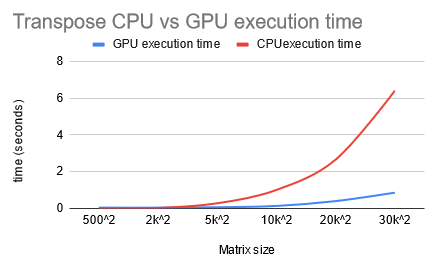
\includegraphics[width=0.45\textwidth]{Transpose_timing.png}
                \captionof{figure}{Transpose Timing Results}
                \label{fig:Transpose Timing}
            \end{center}

        \textbf{End to End Test}\label{End to End Test}\\
            Doing an end to end test of hamc is very simple. You can run the generate executable with the flag "-a test" to run the test suite, and specify each input parameter like such "-n 2 -p 2000 -w 10 -w 120" To run the program with CPU based execution, you pass the "-c" flag. The test suite simply encrypts data, and then decrypts it right away. No input data needs to be given when testing, because randomly generated bits of data are generated for both the GPU and CPU based execution, using the same seed. The seed is by default 10 but can be changed by passing the "-s X" flag where X is the seed value you want. To understand the impact that input parameters have on the workload, the most important parameter is p which determines the dimensions of the square matrix used during all the operations mentioned in Section~\ref{McEliece Operations}.
            
        \begin{center}
            {\rowcolors{2}{green!80!yellow!50}{green!70!yellow!40}
            \begin{tabular}{ | c | c | c | c |} \hline
                \shortstack{input parameters\\(n, p, t, w)} & \shortstack{CPU time\\(minutes)} & \shortstack{GPU time\\(minutes)} & speedup\\ \hline
                2, 2000, 10, 120 & 0.07 & 0.04 & 1.7\\ \hline
                2, 4800, 20, 60 & 7.57 & 1.36 & 5.55\\ \hline
                2, 6000, 20, 60 & 14.78 & 2.26 & 6.53\\ \hline
                2, 1200, 20, 60 & 117.73 & 13.24 & 8.89\\ \hline
                2, 1200, 20, 60 & 938.88 & 70.46 & \textbf{13.32}\\ \hline
                2, 32771, 264, 274 & 938.88+ & N/A & N/A\\ \hline
            \end{tabular}
            }
            \captionof{table}{Timing results for End To End execution}
            \label{fig:E2E_table}
        \end{center}
            
            
        The goal for the end-to-end test was to be able to run the entire program on a matrix of size 32,771 which would offer 256 bits of security\cite{10.1109/ISIT.2013.6620590, 10.1007/978-3-642-29011-4_31}, but unfortunately there is not enough memory on the GPU to store the necessary matrices to do the LU decomposition operations for the inverse. To combat this, blocking LU decomspotion would be the next step, but due to the sake of time, that algorithm was not implemented for this project.
\section{Conclusion}\label{Conclusion}
    \colorbox{yellow}{TODO: conclusion}


\section{Acknowledgement}\label{Acknowledgement}
    We would like to thank Dr. Ali Akoglu for his tremendous support in this project. Without Akoglu's guidance and help, this project would not be where it is. Special thanks to Michael Chuvelev from the Intel OneAPI MKL team for help on the LU decomposition algorithm for inverse.

\printbibliography
\end{document}
